\documentclass{article}
\usepackage{graphicx} % Para incluir imágenes
\usepackage[spanish]{babel}
\usepackage{makeidx}
\usepackage{geometry}
\usepackage{amsmath}
\usepackage{placeins}


\geometry{a4paper, total={170mm,257mm}, left=20mm, top=20mm}


\begin{document}
\begin{titlepage}
    \centering
    \Large
    Universidad Central de Venezuela\\
    Facultad de Ingeniería\\
    Escuela de Ingeniería Eléctrica
    \vspace*{8cm}

    \Huge
    \textbf{Prelaboratorio N° 11: } 

    \textbf{Multivibradores}
    \vfill


    \Large

    Emerson Warhman \\
    C.I. 25.795.480 \\
    \today

\end{titlepage}

\section{Objetivos}

\subsection{Objetivo General}

Analizar el efecto de la Realimentación en el comportamiento de un amplificador.

\subsection{Objetivos Específicos}

\begin{enumerate}
    \item Reconocer que la Realimentación negativa reduce la ganancia y a cambio ofrece:
    \begin{itemize}
        \item Mayor independencia del valor de la ganancia del amplificador base.
        \item Disminución de la impedancia de salida.
        \item Aumento de la impedancia de entrada.
        \item Aumento del ancho de banda.
        \item Mejoramiento de la linealidad del amplificador.
    \end{itemize}
    
\end{enumerate}

\section{Cálculos}

1. Realimente negativamente el amplificador base a través de la entrada diferencial adecuada. Mediante un divisor de tensión $R_f$ y $R_s$.

2. Para el amplificador Realimentado, determine: Puntos de operación de los elementos activos, el modelo dinámico del amplificador y su respuesta en frecuencia, utilizando la entrada libre del diferencial como entrad.


Para realizar los cálculos es necesario conocer los parámetros del amplificador base, los cuales ya fueron determinados en las prácticas anteriores y son los siguientes:

\begin{table}[ht]
\centering
\begin{tabular}{|c|c|c|c|}
        \hline
        \textbf{Transistor} & $I_b$ [$\mu A$] & $I_c$ [$\mu A$] & $V_{CE}$ [$V$] \\ \hline
        $Q_1$ & $2.65$ & $620.00 $ & $7.79$ \\ \hline
        $Q_2$ & $2.65$ & $620.00 $ & $7.79$ \\ \hline
        $Q_3$ & $10.03$ & $2370.00 $ & $2.27$ \\ \hline
        $Q_4$ & $1.31$ & $302.36$ & $1.24$ \\ \hline
        $Q_5$ & $1.52 $ & $350.00$ & $9.99$ \\ \hline
        $Q_6$ & $2.33 $ & $350.00$ & $9.99$ \\ \hline
\end{tabular}
\caption{Puntos de operación del amplificador base}
\end{table}

La ilustración \ref{ilus:amplificador-base} muestra el modelo dinámico del amplificador base. Cuyos parámetros son los mostrados en la tabla \ref{tab:amplificador-base-dinamico}.

\begin{ilustracion}[ht]
    \centering
    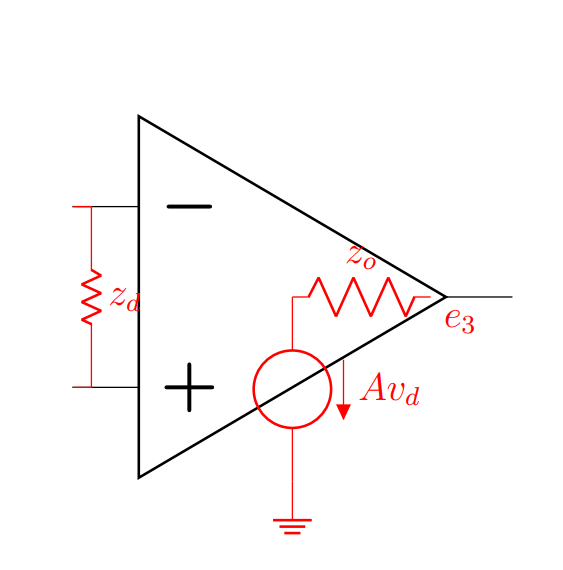
\includegraphics[width=0.6\textwidth]{src/images/modelo-amplificador.png}
    \caption{Modelo dinámico del amplificador base}
    \label{ilus:amplificador-base}
\end{ilustracion}

\begin{table}[ht]
    \centering
    \label{tab:amplificador-base-dinamico}
    \begin{tabular}{|c|c|c|c|}
        \hline
        \textbf{Parámetro} & \textbf{Valor} \\ \hline
        $Z_d$ & $43.99$ [$k\Omega$] \\ \hline
        $Z_o$ & $12.13 $ [$\Omega$] \\ \hline
        $A_b$ & $300$ \\ \hline
        $f_L$ & $69.61$ [$Hz$] \\ \hline
        $f_H$ & $11.00$ [$kHz$] \\ \hline
    \end{tabular}
    \caption{Valores de los parámetros dinámicos del amplificador Realimentado}

\end{table}

Ahora calculamos los parámetros del amplificador realimentado negativamente.\\

para la impedancia de entrada $Z_i$ tenemos:

$$Z_i = R_s = 3.3 k\Omega$$

Y la impedancia de salida viene dada por la expresión:

$$Z_o = \frac{R_o}{A / (1 + \frac{R_f}{R_s})}$$

Por lo tanto el valor de $Z_o$ es:

$$Z_o = 0.137 \Omega$$

El valor de la ganancia de la realimentación negativa es: 

$$A_{fb} = - \frac{R_f}{R_s} = - \frac{11k\Omega}{3.3k\Omega} = -3.33$$

Y debido a que $A => \infty$ en el amplificador base, el valor de la ganancia de la realimentación negativa es:

$$A = -\frac{1}{\beta}$$

despejando $\beta$ de la expresión anterior, tenemos:

$$\beta = -\frac{1}{A} = -\frac{1}{3.33} = 0.333$$

Para encontrar las frecuencias de corte inferior utilizamos la expresión:

$$f_{Lf} = \frac{f_{Lb}}{1 + A_{b}}$$

entonces:

$$f_{Hf} = \frac{69.61 Hz}{1 + 49.54} = 1.37 Hz$$

Para hallar la frecuencia de corte superior utilizamos la expresión:

$$f_{Hf} = f_{Hb}\cdot (1 + A_{b})$$

Por lo tanto:

$$f_{Hf} = 11kHz\cdot (1 + 49.54) = 555.94KHz$$

Ahora, para el amplificador realimentado positivamente, procedemos a calcular la ganancia:

$$A_{fb} = 1 + \frac{R_f}{R_s} = 1 + \frac{11k\Omega}{3.3k\Omega} = 4.33$$

La impedancia de entrada con realimentación positiva es:

$$ Z_i = \frac{Z_d \cdot A_b}{1 + \frac{R_f}{R_s}} = \frac{43.99k\Omega \cdot 300}{1 + \frac{11k\Omega}{3.3k\Omega}} = 3.05M\Omega$$

Y la impedancia de salida con realimentación positiva es igual a la impedancia de salida de realimentación negativa:

$$Z_o = 0.137 \Omega$$

\section{Simulaciones}

La ilustración \ref{ilus:amplificador-realimentado-negativo} muestra el circuito del amplificador realimentado negativamente construido en multisim.

\begin{ilustracion}[ht]
    \centering
    \includegraphics[width=1.0\textwidth]{src/images/Prelaboratorio 5 - Realimentación negativa - circuito.png}
    \caption{Circuito amplificador con realimentación negativa}
    \label{ilus:amplificador-realimentado-negativo}
\end{ilustracion}

En la ilustración \ref{ilus:ganancia-realimentacion-negativa} podemos observar una ganancia de aproximadamente $3.3$ que coincide con la ganancia de los cálculos.

\begin{ilustracion}[ht]
    \centering
    \includegraphics[width=1\textwidth]{src/images/Prelaboratorio 5 - Retroalimentación negativa - Ganancia.png}
    \caption{Ganancia de la realimentación negativa}
    \label{ilus:ganancia-realimentacion-negativa}
\end{ilustracion}

En la ilustración \ref{ilus:respuesta-frecuencia-realimentacion-negativa} podemos observar un aumento en el ancho de banda con realimentación negativa. Podemos observar que las frecuencias de corte coinciden con los cálculados previamente.

\begin{ilustracion}[ht]
    \centering
    \includegraphics[width=1.0\textwidth]{src/images/Prelaboratorio 5 - retroalimentación negativa - respuesta en frecuencia.png}
    \caption{Respuesta en frecuencia del amplificador realimentado negativamente}
    \label{ilus:respuesta-frecuencia-realimentacion-negativa}
\end{ilustracion}

% Realimentación positiva

La ilustración \ref{ilus:circuito-realimentacion-positiva-sin-condensador} muestra la construcción del circuito del amplificador realimentado positivamente.

\begin{ilustracion}[ht]
    \centering
    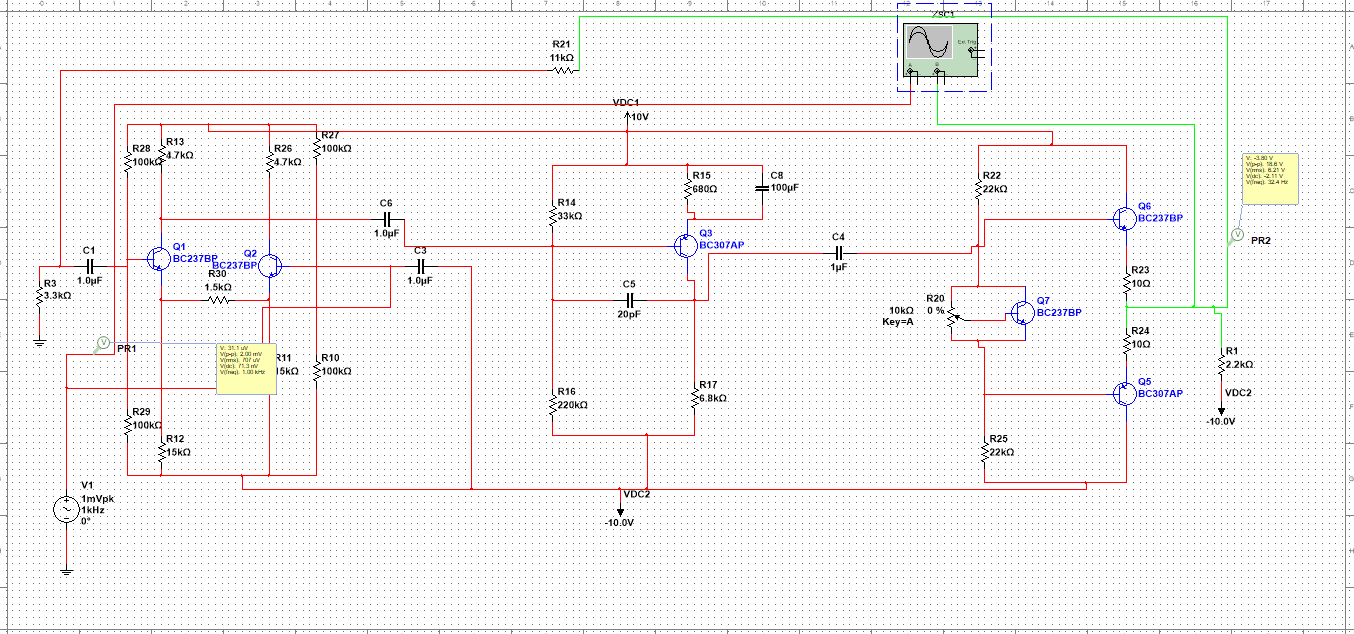
\includegraphics[width=\textwidth]{src/images/Prelaboratorio 5 - Realimentacion positiva sin condensador - circuito.png}
    \caption{Circuito de realimentación positiva sin condensador}
    \label{ilus:circuito-realimentacion-positiva-sin-condensador}
\end{ilustracion}

La ganancia de este amplificador se puede observar en la ilustración del \ref{ilus:ganancia-circuito-realimentacion-positiva-sin-condensador} y podemos observar que coincide con la ganancia calculada anteriormente de 4.33. Sin embargo podemos observar que despues de un tiempo la ganancia cambia y toma la forma mostrada en la ilustración \ref{ilus:ganancia-circuito-realimentacion-positiva-sin-condensador-despues-de-unos-segundos}.

\begin{ilustracion}[ht]
    \centering
    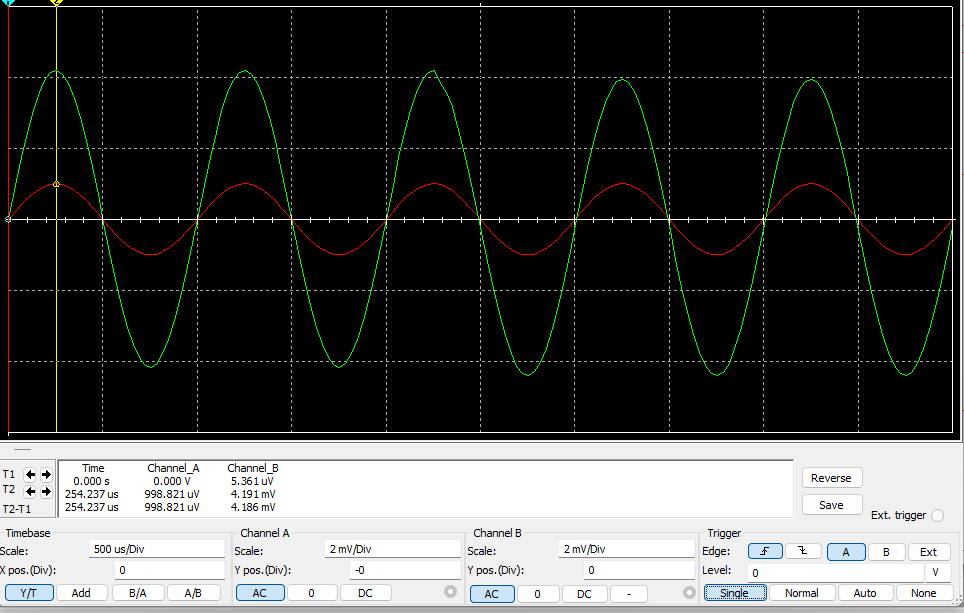
\includegraphics[width=\textwidth]{src/images/Prelaboratorio 5 - Realimentacion positiva sin condensador - ganancia.png}
    \caption{Ganancia del circuito de realimentación positiva sin condensador}
    \label{ilus:ganancia-circuito-realimentacion-positiva-sin-condensador}
\end{ilustracion}


\begin{ilustracion}[ht]
    \centering
    \includegraphics[width=\textwidth]{src/images/Prelaboratorio 5 - Retroalimentación positiva sin condensador despues de unos segundos.png}
    \caption{Ganancia del circuito de realimentación positiva sin condensador despues de unos segundos}
    \label{ilus:ganancia-circuito-realimentacion-positiva-sin-condensador-despues-de-unos-segundos}
\end{ilustracion}

Podemos observar la respuesta en frecuencia del amplificador realimentado positivamente en la ilustración \ref{ilus:respuesta-amplificador-realimentacion-positiva-sin-condensador}.

\begin{ilustracion}[ht]
    \centering
    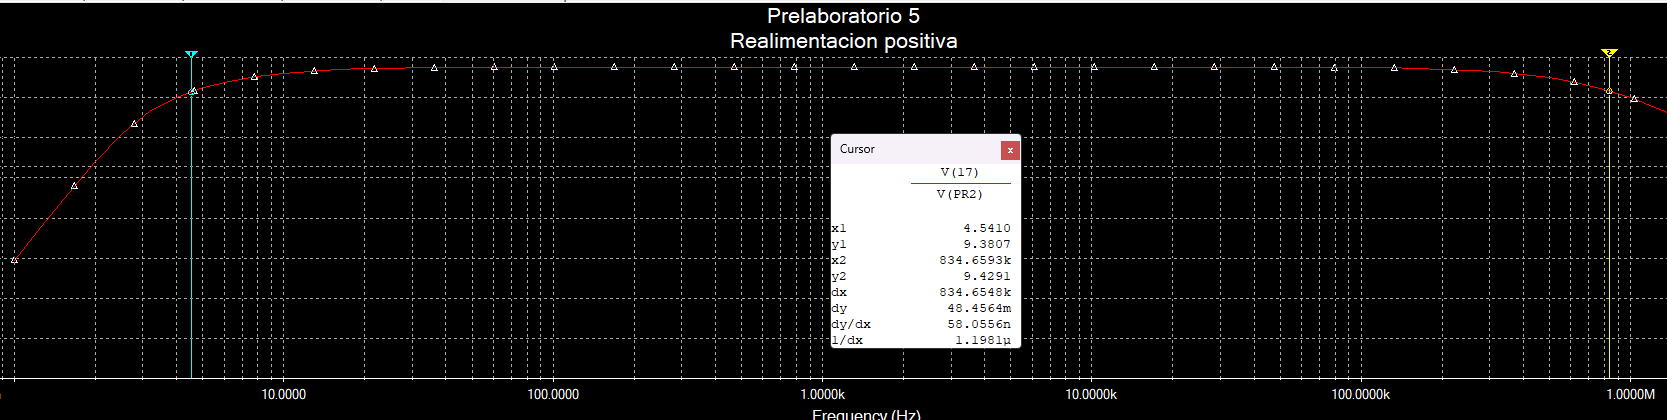
\includegraphics[width=\textwidth]{src/images/Prelaboratorio 5 - realimentacion positiva sin condensador - respuesta en frecuencia.png}
    \caption{Respuesta en frecuencia del amplificador con Realimentación positiva sin condensador} 
    \label{ilus:respuesta-amplificador-realimentacion-positiva-sin-condensador}
\end{ilustracion}

% Amplificador realimentado positiva y negativamente

La ilustración \ref{ilus:circuito-amplificador-realimentacion-positiva-y-negativa} muestra el circuito del amplificador con realimentación positiva y negativa con condensador.

\begin{ilustracion}[ht]
    \centering
    \includegraphics[width=\textwidth]{src/images/prelaboratorio 5 - circuito realimentación positiva con condensador.png}
    \caption{Circuito con realimentación positiva y negativa} 
    \label{ilus:circuito-amplificador-realimentacion-positiva-y-negativa}
\end{ilustracion}

La ganancia este amplificador se puede observar en la ilustración \ref{ilus:ganancia-amplificador-realimentacion-positiva-y-negativa}.
\begin{ilustracion}[ht]
    \centering
    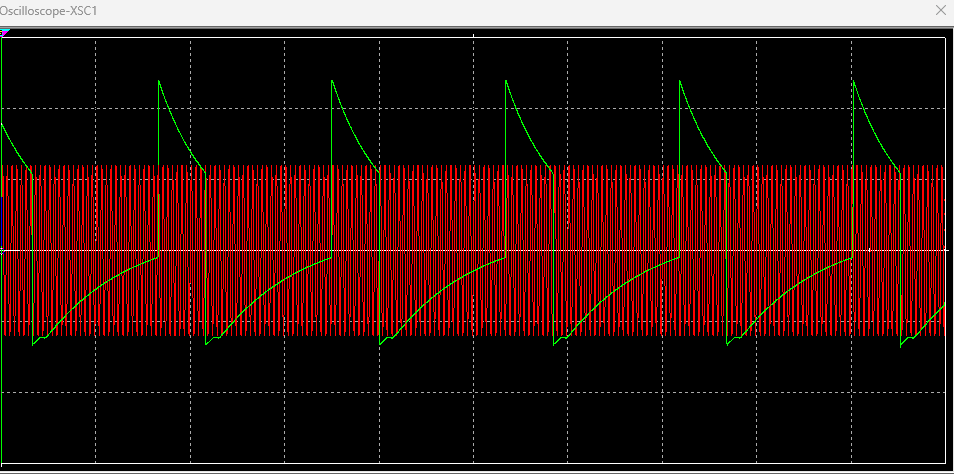
\includegraphics[width=\textwidth]{src/images/Prelaboratorio 5 - Ganancia realimentacion positiva con condensador.png}
    \caption{Ganancia con realimentación positiva y negativa} 
    \label{ilus:ganancia-amplificador-realimentacion-positiva-y-negativa}
\end{ilustracion}

La respuesta en frecuencia del amplificador se puede observar en la ilustración \ref{ilus:respuesta-amplificador-realimentacion-positiva-y-negativa}.

\begin{ilustracion}[ht]
    \centering
    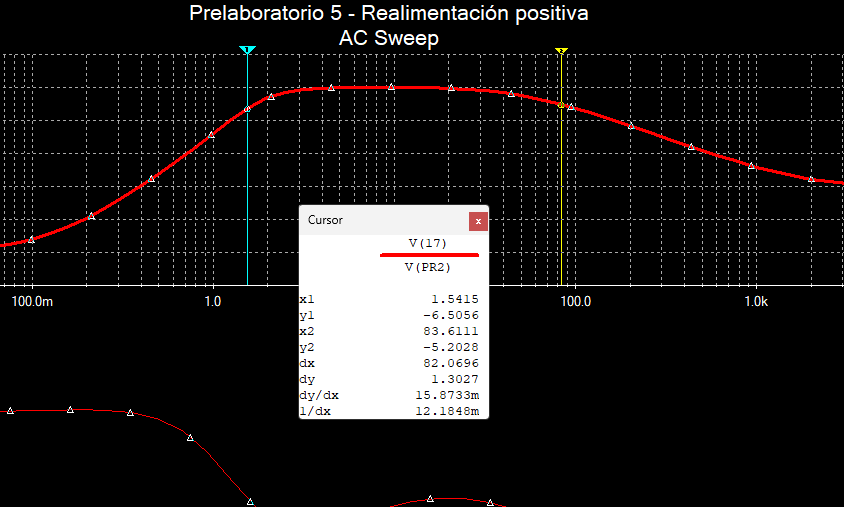
\includegraphics[width=\textwidth]{src/images/Prelaboratorio 5 - Respuesta en frecuencia - realimentacion positiva con condensador.png}
    \caption{Circuito con realimentación positiva y negativa} 
    \label{ilus:respuesta-amplificador-realimentacion-positiva-y-negativa}
\end{ilustracion}

\FloatBarrier

\section{Metodología}

En la práctica de laboratorio se realizará el siguiente procedimiento:

\begin{enumerate}
    \item Se realiza el montaje del amplificador base (sin realimentación).
    \item Se tomarán las mediciones de los puntos estáticos de operación de los elementos activos sin haber conectado la fuente AC.
    \item Con la fuente AC conectada, se medirá la impedancia de salida e impedancia de entrada utilizando las resistencias patrón $R_{pi} = 43k\Omega$ y $R_{po}=10\Omega$.
    \item Se medirá la ganancia a frecuencias medias midiendo el voltaje de entrada y el voltaje de salida.
    \item Se medirán las frecuencias de corte calculando $\frac{A}{0.707}$ y ajustando la frecuencia del generador de ondas hasta que la medición del voltaje de salida coincida con el valor calculado tanto para bajas frecuencias como para altas frecuencias.
    \item Se ajustará la polarización de la etapa de potencia para convertirla en una clase C y se tomará foto del efecto crossover en la señal de salida.
    \item Se realimentará el amplificador base con  una red divisor de tensión con las resistencias $R_s= 3.3k\Omega$ y $R_f= 11k\Omega$. Se observará el efecto crossover y se tomará una fotografía.
    \item Para el amplificador realimentado negativamente se determinará las impedancias de entrada y de salida, la ganancia a frecuencias medias, las frecuencias de corte superior e inferior utlizando la misma metodologías que en los pasos 3 a 5.
    \item Se medirá la respuesta en frecuencia tomando un muestreo variando la frecuencia del generador a valores cercanos a las frecuencias de corte y a la frecuencia de máxima amplitud.
    \item Se conectará la realimentación positiva conectando ademas una conexión con otra resistencia $11k\Omega$ y el condensador de $10nF$ y se tomará una fotografía. 
\end{enumerate}


\end{document}
